\section{Beziehung zwischen Julia-Mengen und Mandelbrot-Menge}
\label{julia:sec:relation}
\kopfrechts{Beziehung zwischen Julia-Mengen und Mandelbrot-Menge}%

Zwischen der Mandelbrot-Menge sowie den Julia- bzw. Fatou-Mengen bestehen mehrere, teils überraschende Zusammenhänge.
In diesem Abschnitt werden drei solche Zusammenhänge näher betrachtet.

\subsection{Form der Julia-Mengen}
\label{julia:sec:julia_connected}
Anhand der Position in der Mandelbrot-Menge, lässt sich eine Aussage über die Form bzw. das Aussehen der zugehörigen Julia-Menge treffen.
Dafür werden stets Funktionen der Art $f_c(z) = z^2 + c$ betrachtet.

Setzt man zunächst $c = 0$, befindet man sich in der Abbildung \ref{julia:fig:mandelbrot_julia_1} beim weissen Punkt in der Mandelbrot-Menge links.
Rechts daneben ist die Julia-Menge der Funktion $f_c(z) = z^2 + 0$ dargestellt, wobei es sich bekanntlich um den Rand des Einheitskreises handelt.

\begin{figure}
    \centering
    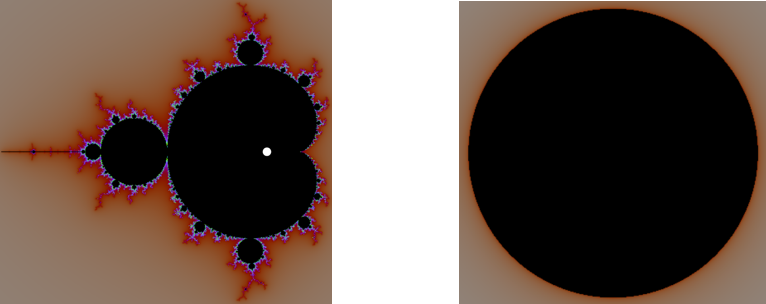
\includegraphics[width=\textwidth]{papers/julia/imgs/mandelbrot_julia_1.png}
    \caption{Mandelbrot-Menge bei $c=0$ und zugehörige Julia-Menge}
    \label{julia:fig:mandelbrot_julia_1}
\end{figure}

Verschiebt man nun $c$ entlang der imaginären Achse, erhält man die Folge von Bildern in den Abbildungen \ref{julia:fig:mandelbrot_julia_2-4} und \ref{julia:fig:mandelbrot_julia_5}.
Links ist jeweils die aktuelle Position des Punktes $c$ dargestellt und rechts die Julia-Menge der Funktion $f_c$ --- parametrisiert mit dem aktuellen $c$.

\begin{figure}
    \centering
    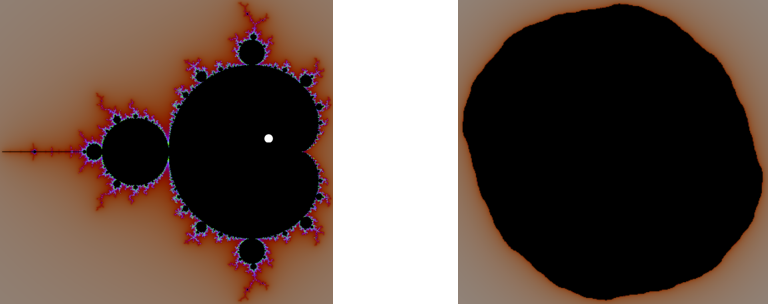
\includegraphics[width=\textwidth]{papers/julia/imgs/mandelbrot_julia_2.png}
    \\[\smallskipamount]
    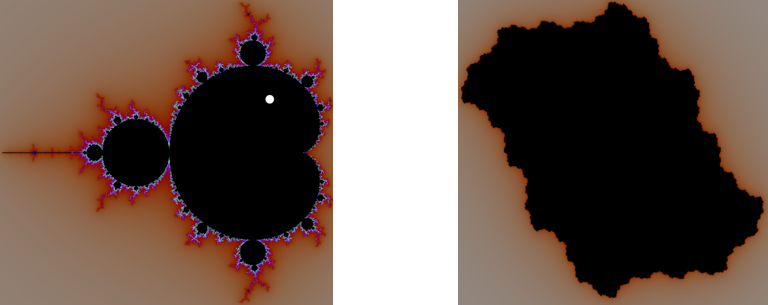
\includegraphics[width=\textwidth]{papers/julia/imgs/mandelbrot_julia_3.png}
    \\[\smallskipamount]
    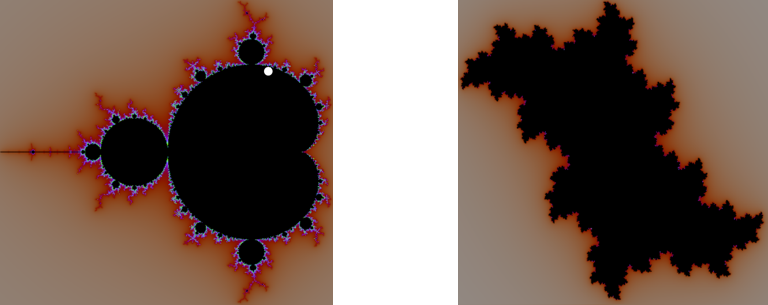
\includegraphics[width=\textwidth]{papers/julia/imgs/mandelbrot_julia_4.png}

    \caption{Mandelbrot-Menge bei $c \in \{\,0.1i,\, 0.4i,\, 0.6i\,\}$ und zugehörige Julia-Mengen}
    \label{julia:fig:mandelbrot_julia_2-4}
\end{figure}

\begin{figure}
    \centering
    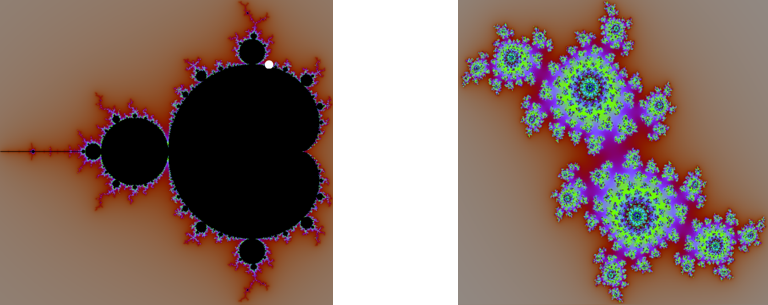
\includegraphics[width=\textwidth]{papers/julia/imgs/mandelbrot_julia_5.png}

    \caption{Mandelbrot-Menge bei $c = 0.65i$, ausserhalb von $M$ und zugehörige Julia-Menge}
    \label{julia:fig:mandelbrot_julia_5}
\end{figure}

Mit änderndem $c$ verformt sich die Julia-Menge zusehends und beim Übergang von $c=0.6i$ zu $c=0.65i$ zerfällt sie.
Grund dafür ist, dass $c=0.6i$ noch in der Mandelbrot-Menge $M$ liegt, während $c=0.65i$ bereits ausserhalb ist.
In den Abbildungen \ref{julia:fig:mandelbrot_julia_2-4} und \ref{julia:fig:mandelbrot_julia_5} ist die Mandelbrot-Menge schwarz dargestellt, alle eingefärbten Punkte gehören nicht mehr dazu.

Es stellt sich heraus, dass die Julia-Menge \emph{zusammenhängend} ist, für alle $c \in M$ und \emph{nicht zusammenhängend} für alle $c \not\in M$.
\index{zusammenhangend@zusammenhängend}%


\subsection{Ähnlichkeit der Mandelbrot- und Julia-Menge}
In der Vergangenheit wurde mehrfach beobachtet, dass Strukturen in der Mandelbrot-Menge ganzen Julia-Mengen ähneln.
Wie sich ergab, tritt für gewisse Arten von Parametern $c$ ein interessantes Phänomen auf.
Dies soll an Funktionen der Art $f_c(z) = z^2 + c$ illustriert werden.

\begin{beispiel}
    Nachfolgend wird der Punkt \[c_1 = 0.3626697754647427\, +\, 0.6450273437137847i\] betrachtet.
    Vergrössert man die Mandelbrot-Menge an diesem Punkt, so ergibt sich die Reihe von Bildern in Abbildung \ref{julia:fig:mandelbrot_zoom}.

    \begin{figure}
        \centering
        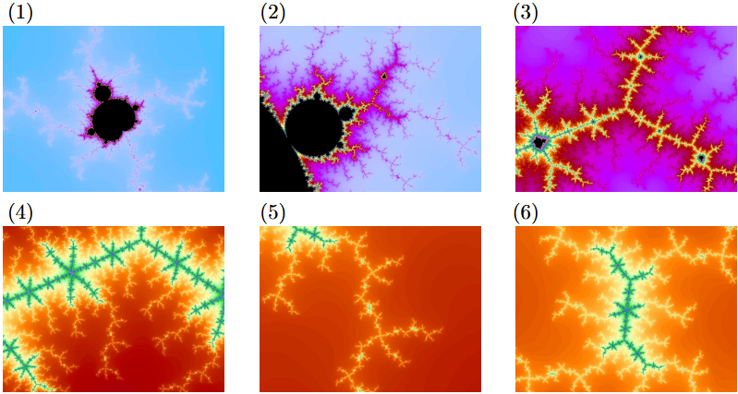
\includegraphics[width=\textwidth]{papers/julia/imgs/mandelbrot_zoom.png}

        \caption{Zoom der Mandelbrot-Menge bei $c_1 = 0.3626697754647427 + 0.6450273437137847i$, vgl. mit Abbildung \ref{julia:fig:julia_zoom} (2)}
        \label{julia:fig:mandelbrot_zoom}
    \end{figure}

    Macht man das gleiche mit der Julia-Menge der Funktion \[f = z^2\, +\, 0.3626697754647427\, +\, 0.6450273437137847i\] ergeben sich die Bilder in Abbildung \ref{julia:fig:julia_zoom}.

    \begin{figure}
        \centering
        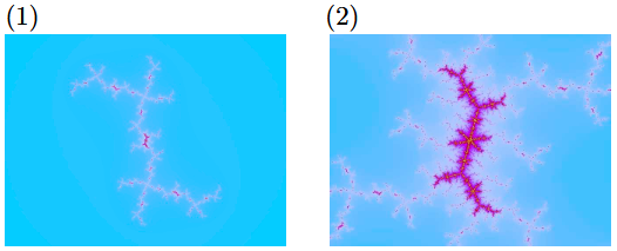
\includegraphics[width=0.65\textwidth]{papers/julia/imgs/julia_zoom.png}

        \caption{Julia-Menge von $f(z) = z^2 + 0.3626697754647427 + 0.6450273437137847i$, vgl. mit Abbildung \ref{julia:fig:mandelbrot_zoom} (6)}
        \label{julia:fig:julia_zoom}
    \end{figure}

    Bis auf das Farbschema und die Ausrichtung sind sind die Bilder (6) der Mandelbrot-Menge und (2) der Julia-Menge fast gleich.
\end{beispiel}

Wie Kawahira und Kisaka in \cite{julia:ähnlichkeit_mandelbrot} gezeigt haben, passiert dies für parabolische Parameter und Misiurewicz-Parameter.
\begin{definition}
    Ein Parameter $c$ wird als \emph{parabolisch} bezeichnet, wenn die Funktion $f_c$ einen periodischen Punkt besitzt, dessen Multiplikator $\lambda$ \eqref{julia:lambda_multiplicator} eine Einheitswurzel (siehe \ref{julia:sec:nicht_fix_periodisch}) ist.
\index{parabolischer Parameter}%
\index{Parameter!parabolisch}%
\end{definition}
\begin{beispiel}
    Ein Beispiel ist der Parameter $c = \frac{1}{4}$.
    Die Funktion $f(z) = z^2 + \frac{1}{4}$ besitzt einen Fixpunkt bei $z_0 = \frac{1}{2}$, denn $f(z_0) = \left(\frac{1}{2}\right)^2 + \frac{1}{4} = z_0$.
    Weiter ist $\lambda = \left(f\right)^\prime(z_0) = 2 z_0 = 1$, wobei es sich um eine Einheitswurzel handelt.
\end{beispiel}

\begin{definition}
    Ein Parameter $c$ heisst \emph{Misiurewicz-Parameter}, wenn der Startwert $z_0 = 0$ präperiodisch, aber nicht periodisch ist.
\index{Misiurewicz-Parameter}%
\index{Parameter!Misiurewicz-}%
\end{definition}
Ein präperiodischer Startwert wird nach endlich vielen Iterationen periodisch, ist aber selbst nicht periodisch.
Dies ist dargestellt in Abbildung \ref{julia:fig:preperiodic}.

\begin{figure}
    \centering
    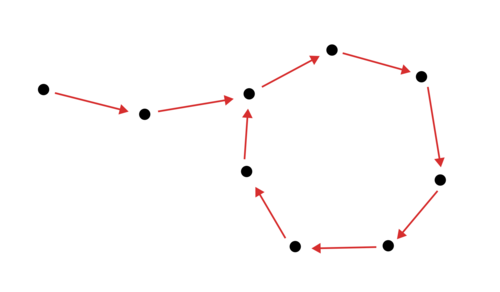
\includegraphics[width=0.6\textwidth]{papers/julia/imgs/preperiodic.png}

    \caption{Ein Zyklus ausgehend von einem präperiodischen Startwert}
    \label{julia:fig:preperiodic}
\end{figure}

\begin{beispiel}
    Beim Parameter $c = -2$ handelt es sich um einen Misiurewicz-Parameter, iteriert man die Funktion $f_c$ ausgehend von $z_0 = 0$, ergibt sich die Folge
    \begin{equation*}
        0 \mapsto -2 \mapsto 2 \mapsto 2 \mapsto 2 \mapsto \ldots\, .
    \end{equation*}
    Diese Folge wird ab der dritten Iteration periodisch.
\end{beispiel}


\subsection{Mosaik der Mandelbrot-Menge}
Werden Julia-Mengen auf eine bestimmte Art angeordnet, ergibt sich ein Mosaik der Mandelbrot-Menge.
Dazu legt man ein Gitter über die Mandelbrot-Menge und wählt einen Gitterpunkt aus, illustriert in der Abbildung \ref{julia:fig:mosaik1}.

\begin{figure}
    \centering
    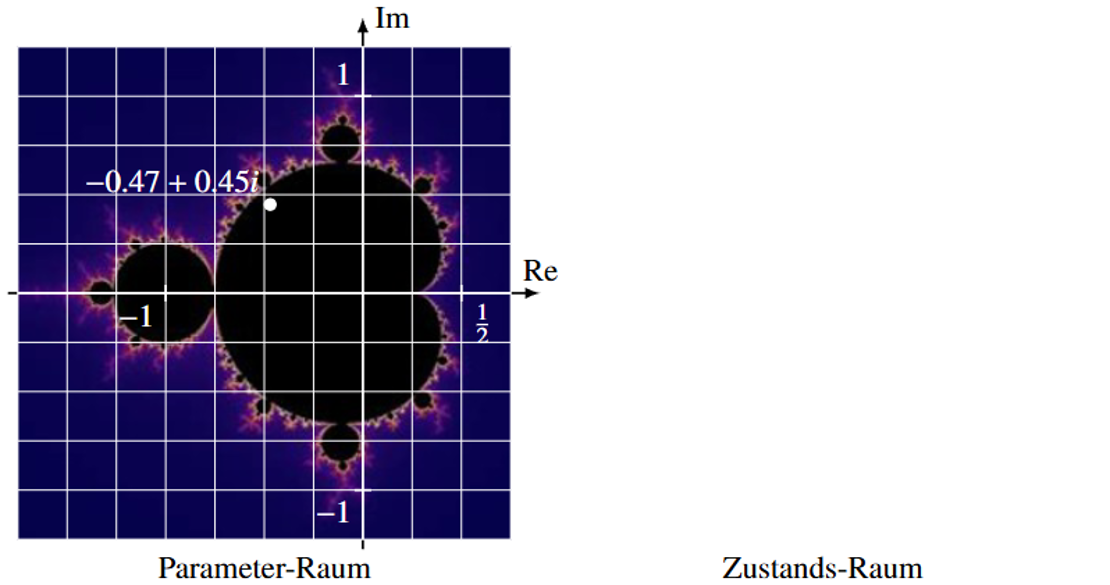
\includegraphics[width=0.95\textwidth]{papers/julia/imgs/mosaik1.png}

    \caption{Gitterpunkt $-0.47 + 0.45i$ in der Mandelbrot-Menge}
    \label{julia:fig:mosaik1}
\end{figure}

Mit dem gewählten Parameter $c = -0.47 + 0.45i$ berechnet man nun die Julia-Menge der Funktion $f(z) = z^2 - 0.47 + 0.45i$.
Die Julia-Menge wird nun in das Gitter platziert und zwar an den Ort des Parameters $c$.
Anschliessend wird sie verkleinert, dies ist in Abbildung \ref{julia:fig:mosaik2-4} dargestellt.
Nun wird dieser Vorgang für sämtliche Gitterpunkte wiederholt, wodurch Abbildung \ref{julia:fig:mosaik5} entsteht.

\begin{figure}
    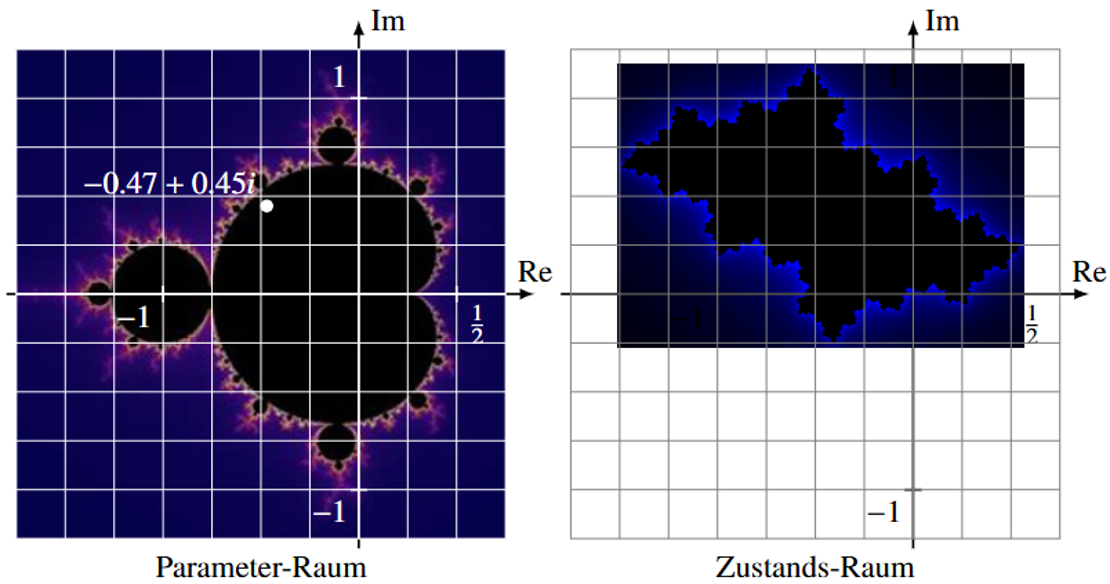
\includegraphics[width=0.95\textwidth]{papers/julia/imgs/mosaik2.png}
    \\[\smallskipamount]
    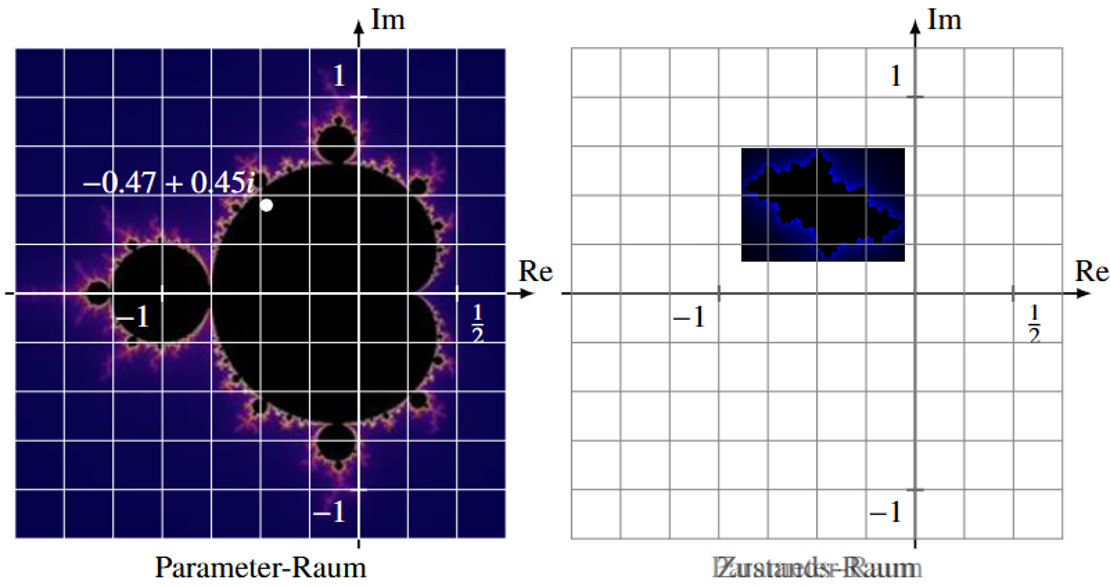
\includegraphics[width=0.95\textwidth]{papers/julia/imgs/mosaik3.png}
    \\[\smallskipamount]
    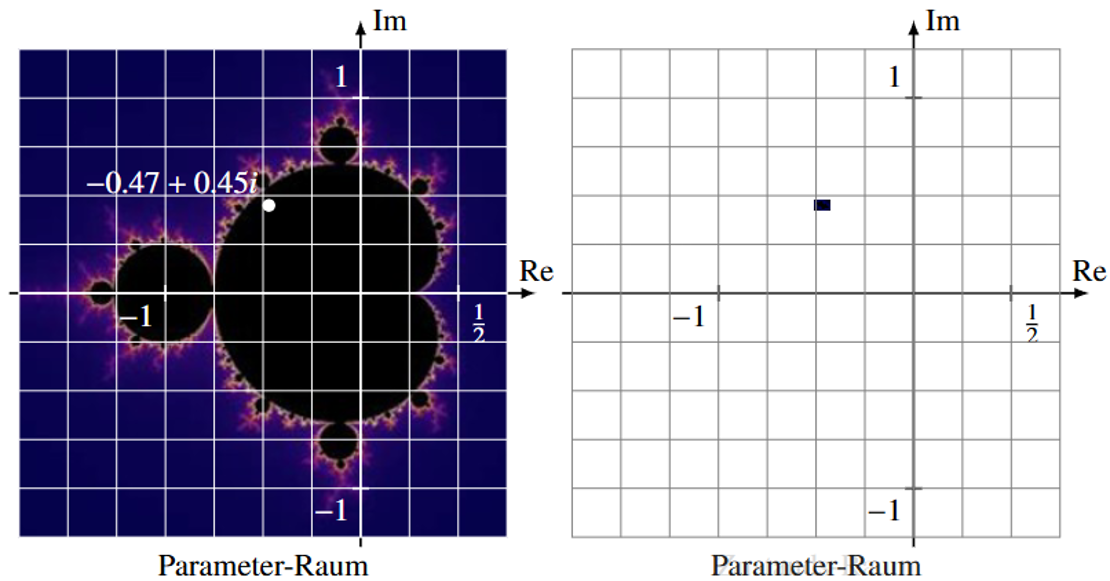
\includegraphics[width=0.95\textwidth]{papers/julia/imgs/mosaik4.png}

    \caption{Kleiner werdende Julia-Menge der Funktion $f(z) = z^2 - 0.47 + 0.45i$ am Punkt $-0.47 + 0.45i$}
    \label{julia:fig:mosaik2-4}
\end{figure}

\begin{figure}
    \centering
    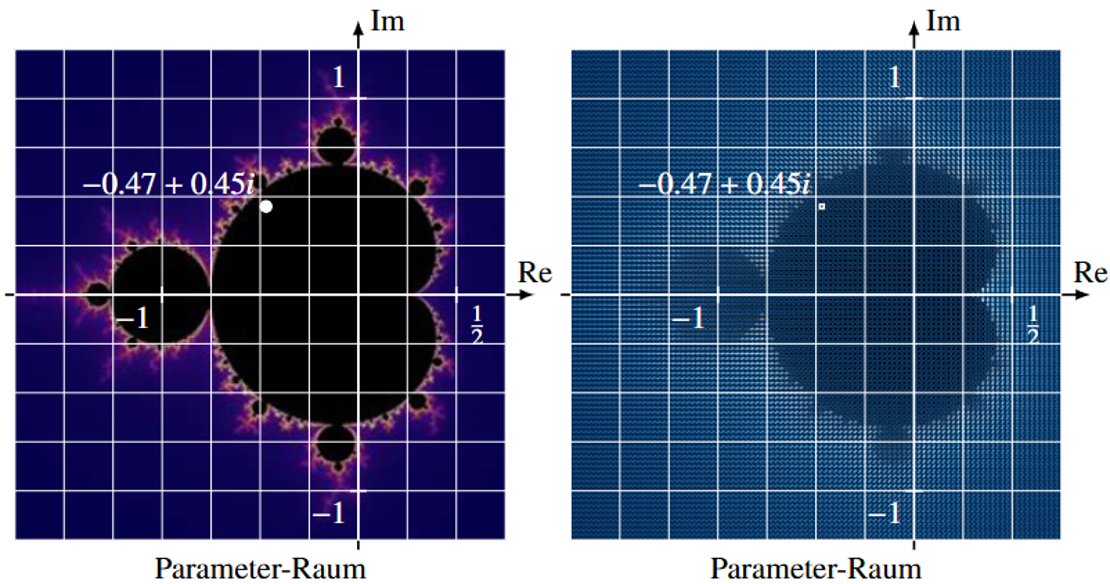
\includegraphics[width=0.95\textwidth]{papers/julia/imgs/mosaik5.png}

    \caption{Mosaik der Mandelbrot-Menge bestehend aus $100$ mal $100$ Julia-Mengen}
    \label{julia:fig:mosaik5}
\end{figure}

Aus dem Zustandsraum, in dem die Julia-Mengen existieren, wurde der Parameterraum nachgestellt, in dem die Mandelbrot-Menge existiert.
Der Grund für dieses Resultat ist, dass die Mandelbrot-Menge eine Art ``Katalog'' sämtlicher Julia-Mengen bildet.
